\chapter{Combat}
\section{How Combat Works}

\label{f0}				
Combat is cyclical; everybody acts in turn in a regular cycle of rounds. Combat follows this sequence:
				
1. When combat begins, all combatants roll initiative.
				
2. Determine which characters are aware of their opponents. These characters can act during a surprise round. If all the characters are aware of their opponents, proceed with normal rounds. See the surprise section for more information.
				
3. After the surprise round (if any), all combatants are ready to being the first normal round of combat.
				
4. Combatants act in initiative order (highest to lowest).
				
5. When everyone has had a turn, the next round begins with the combatant with the highest initiative, and steps 4 and 5 repeat until combat ends.
				
\subsection{The Combat Round}

				
Each round represents 6 seconds in the game world; there are 10 rounds in a minute of combat. A round normally allows each character involved in a combat situation to act. 
				
Each round's activity begins with the character with the highest initiative result and then proceeds in order. When a character's turn comes up in the initiative sequence, that character performs his entire round's worth of actions. (For exceptions, see Attacks of Opportunity and Special Initiative Actions.)
				
When the rules refer to a \texttt{{}"{}}full round\texttt{{}"{}}, they usually mean a span of time from a particular initiative count in one round to the same initiative count in the next round. Effects that last a certain number of rounds end just before the same initiative count that they began on.
				
\subsection{Initiative}

				
At the start of a battle, each combatant makes an initiative check. An initiative check is a Dexterity check. Each character applies his or her Dexterity modifier to the roll, as well as other modifiers from feats, spells, and other effects. Characters act in order, counting down from the highest result to the lowest. In every round that follows, the characters act in the same order (unless a character takes an action that results in his or her initiative changing; see Special Initiative Actions).
				
If two or more combatants have the same initiative check result, the combatants who are tied act in order of total initiative modifier (highest first). If there is still a tie, the tied characters should roll to determine which one of them goes before the other.
				
\textbf{Flat-Footed}: At the start of a battle, before you have had a chance to act (specifically, before your first regular turn in the initiative order), you are flat-footed. You can't use your Dexterity bonus to AC (if any) while flat-footed. Barbarians and rogues of high enough level have the uncanny dodge extraordinary ability, which means that they cannot be caught flat-footed. Characters with uncanny dodge retain their Dexterity bonus to their AC and can make attacks of opportunity before they have acted in the first round of combat. A flat-footed character can't make attacks of opportunity, unless he has the Combat Reflexes feat.
				
\textbf{Inaction}: Even if you can't take actions, you retain your initiative score for the duration of the encounter.
				
\subsection{Surprise}

				
When a combat starts, if you are not aware of your opponents and they are aware of you, you're surprised.
				
Sometimes all the combatants on a side are aware of their opponents, sometimes none are, and sometimes only some of them are. Sometimes a few combatants on each side are aware and the other combatants on each side are unaware.
				
Determining awareness may call for Perception checks or other checks.
				
\textbf{The Surprise Round}: If some but not all of the combatants are aware of their opponents, a surprise round happens before regular rounds begin. In initiative order (highest to lowest), combatants who started the battle aware of their opponents each take a standard or move action during the surprise round. You can also take free actions during the surprise round. If no one or everyone is surprised, no surprise round occurs.
				
\textbf{Unaware Combatants}: Combatants who are unaware at the start of battle don't get to act in the surprise round. Unaware combatants are flat-footed because they have not acted yet, so they lose any Dexterity bonus to AC.
				
\section{Combat Statistics}

				
This section summarizes the statistics that determine success in combat, then details how to use them.
				
\subsection{Attack Roll}

				
An attack roll represents your attempt to strike your opponent on your turn in a round. When you make an attack roll, you roll a d20 and add your attack bonus. (Other modifiers may also apply to this roll.) If your result equals or beats the target's Armor Class, you hit and deal damage.
				
\textbf{Automatic Misses and Hits}: A natural 1 (the d20 comes up 1) on an attack roll is always a miss. A natural 20 (the d20 comes up 20) is always a hit. A natural 20 is also a threat---a possible critical hit (see the attack action).
				
\subsection{Attack Bonus}

				
Your attack bonus with a melee weapon is the following:
				
{\large \textbf{Base attack bonus + Strength modifier + size modifier}}
				
With a ranged weapon, your attack bonus is the following:
				
{\large \textbf{Base attack bonus + Dexterity modifier + size modifier + range penalty}}
								
\subsection{Armor Class}

				
Your Armor Class (AC) represents how hard it is for opponents to land a solid, damaging blow on you. It's the attack roll result that an opponent needs to achieve to hit you. Your AC is equal to the following: 
				
{\large \textbf{10 + armor bonus + shield bonus + Dexterity modifier + other modifiers}}
				
Note that armor limits your Dexterity bonus, so if you're wearing armor, you might not be able to apply your whole Dexterity bonus to your AC (see Table: Armor and Shields).
				
Sometimes you can't use your Dexterity bonus (if you have one). If you can't react to a blow, you can't use your Dexterity bonus to AC. If you don't have a Dexterity bonus, your AC does not change.
				
\textbf{Other Modifiers}: Many other factors modify your AC.
				
\textit{Enhancement Bonuses}: Enhancement bonuses apply to your armor to increase the armor bonus it provides.
				
\textit{Deflection Bonus}: Magical deflection effects ward off attacks and improve your AC.
				
\textit{Natural Armor}: If your race has a tough hide, scales, or thick skin you receive a bonus to your AC.
				
\textit{Dodge Bonuses}: Dodge bonuses represent actively avoiding blows. Any situation that denies you your Dexterity bonus also denies you dodge bonuses. (Wearing armor, however, does not limit these bonuses the way it limits a Dexterity bonus to AC.) Unlike most sorts of bonuses, dodge bonuses stack with each other.
% <
\begin{table}[]
\sffamily
\caption{Table: Size Modifiers}
\begin{tabular}{ll}
\textbf{Size} & \textbf{Size Modifier}\\
Colossal & --8 \\
 Gargantuan & --4 \\
 Huge & --2 \\
 Large & --1 \\
 Medium & +0 \\
 Small & +1 \\
 Tiny & +2 \\
 Diminutive & +4 \\
 Fine & +8\\
\end{tabular}
\end{table}

				
\textit{Size Modifier}: You receive a bonus or penalty to your AC based on your size. See Table: Size Modifiers.
				
\textbf{Touch Attacks}: Some attacks completely disregard armor, including shields and natural armor---the aggressor need only touch a foe for such an attack to take full effect. In these cases, the attacker makes a touch attack roll (either ranged or melee). When you are the target of a touch attack, your AC doesn't include any armor bonus, shield bonus, or natural armor bonus. All other modifiers, such as your size modifier, Dexterity modifier, and deflection bonus (if any) apply normally. Some creatures have the ability to make incorporeal touch attacks. These attacks bypass solid objects, such as armor and shields, by passing through them. Incorporeal touch attacks work similarly to normal touch attacks except that they also ignore cover bonuses. Incorporeal touch attacks do not ignore armor bonuses granted by force effects, such as \textit{mage armor} and \textit{bracers of armor}.
				
\subsection{Damage}

				
If your attack succeeds, you deal damage. The type of weapon used determines the amount of damage you deal. 
				
Damage reduces a target's current hit points.
				
\textbf{Minimum Damage}: If penalties reduce the damage result to less than 1, a hit still deals 1 point of nonlethal damage.
				
\textbf{Strength Bonus}: When you hit with a melee or thrown weapon, including a sling, add your Strength modifier to the damage result. A Strength penalty, but not a bonus, applies on damage rolls made with a bow that is not a composite bow.
				
\textit{Off-Hand Weapon}: When you deal damage with a weapon in your off hand, you add only 1/2 your Strength bonus. If you have a Strength penalty, the entire penalty applies.
				
\textit{Wielding a Weapon Two-Handed}: When you deal damage with a weapon that you are wielding two-handed, you add 1-1/2 times your Strength bonus (Strength penalties are not multiplied). You don't get this higher Strength bonus, however, when using a light weapon with two hands.
				
\textbf{Multiplying Damage}: Sometimes you multiply damage by some factor, such as on a critical hit. Roll the damage (with all modifiers) multiple times and total the results. 
				
\textit{Note}: When you multiply damage more than once, each multiplier works off the original, unmultiplied damage. So if you are asked to double the damage twice, the end result is three times the normal damage.
				
\textit{Exception}: Extra damage dice over and above a weapon's normal damage are never multiplied.
				
\textbf{Ability Damage}: Certain creatures and magical effects can cause temporary or permanent ability damage (a reduction to an ability score).
				
\subsection{Hit Points}

				
When your hit point total reaches 0, you're disabled. When it reaches --1, you're dying. When it gets to a negative amount equal to your Constitution score, you're dead. See Injury and Death, for more information.
				
\subsection{Attacks of Opportunity}

				
Sometimes a combatant in a melee lets her guard down or takes a reckless action. In this case, combatants near her can take advantage of her lapse in defense to attack her for free. These free attacks are called attacks of opportunity. See the Attacks of Opportunity diagram for an example of how they work.
				
\textbf{Threatened Squares}: You threaten all squares into which you can make a melee attack, even when it is not your turn. Generally, that means everything in all squares adjacent to your space (including diagonally). An enemy that takes certain actions while in a threatened square provokes an attack of opportunity from you. If you're unarmed, you don't normally threaten any squares and thus can't make attacks of opportunity.
				
\textit{Reach Weapons}: Most creatures of Medium or smaller size have a reach of only 5 feet. This means that they can make melee attacks only against creatures up to 5 feet (1 square) away. However, Small and Medium creatures wielding reach weapons threaten more squares than a typical creature. In addition, most creatures larger than Medium have a natural reach of 10 feet or more.
				
\textbf{Provoking an Attack of Opportunity}: Two kinds of actions can provoke attacks of opportunity: moving out of a threatened square and performing certain actions within a threatened square.
				
\textit{Moving}: Moving out of a threatened square usually provokes attacks of opportunity from threatening opponents. There are two common methods of avoiding such an attack---the 5-foot step and the withdraw action.
				
\textit{Performing a Distracting Act}: Some actions, when performed in a threatened square, provoke attacks of opportunity as you divert your attention from the battle. Table: Actions in Combat notes many of the actions that provoke attacks of opportunity.
				
Remember that even actions that normally provoke attacks of opportunity may have exceptions to this rule.
				
\textbf{Making an Attack of Opportunity}: An attack of opportunity is a single melee attack, and most characters can only make one per round. You don't have to make an attack of opportunity if you don't want to. You make your attack of opportunity at your normal attack bonus, even if you've already attacked in the round.
				
An attack of opportunity \texttt{{}"{}}interrupts\texttt{{}"{}} the normal flow of actions in the round. If an attack of opportunity is provoked, immediately resolve the attack of opportunity, then continue with the next character's turn (or complete the current turn, if the attack of opportunity was provoked in the midst of a character's turn).
				
\textit{Combat Reflexes and Additional Attacks of Opportunity}: If you have the Combat Reflexes feat, you can add your Dexterity bonus to the number of attacks of opportunity you can make in a round. This feat does not let you make more than one attack for a given opportunity, but if the same opponent provokes two attacks of opportunity from you, you could make two separate attacks of opportunity (since each one represents a different opportunity). Moving out of more than one square threatened by the same opponent in the same round doesn't count as more than one opportunity for that opponent. All these attacks are at your full normal attack bonus.

\begin{figure}
\sffamily
\caption{Attacks of Opportunity}
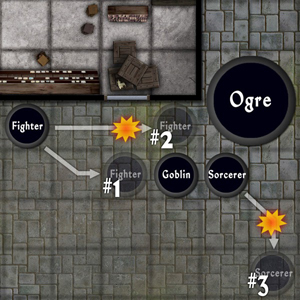
\includegraphics[width=\linewidth]{images/AttacksOfOpportunity.jpg}

In this combat, the fighter and the sorcerer fight an ogre and his goblin buddy.\newline
\#1: The fighter can safely approach this way without provoking an attack of opportunity, as he does not pass through a square threatened by the ogre (who has 10 feet of reach) or the goblin.\newline
\#2: If the fighter approaches this way, he provokes two attacks of opportunity since he passes through a square both creatures threaten.\\
\#3: The sorcerer moves away using a withdraw action. The first square she leaves is not threatened as a result, and she can thus move away from the goblin safely, but when she leaves the second square, she provokes an attack of opportunity from the ogre (who has 10 feet of reach). She could instead limit her movement to a 5-foot step, as a free action, and not provoke any attacks of opportunity.\\
\end{figure}

				
\subsection{Speed}

				
Your speed tells you how far you can move in a round and still do something, such as attack or cast a spell. Your speed depends mostly on your size and your armor.
				
Dwarves, gnomes, and halflings have a speed of 20 feet (4 squares), or 15 feet (3 squares) when wearing medium or heavy armor (except for dwarves, who move 20 feet in any armor).
				
Humans, elves, half-elves, half-orcs, and most humanoid monsters have a speed of 30 feet (6 squares), or 20 feet (4 squares) in medium or heavy armor.
				
If you use two move actions in a round (sometimes called a \texttt{{}"{}}double move\texttt{{}"{}} action), you can move up to double your speed. If you spend the entire round running, you can move up to quadruple your speed (or triple if you are in heavy armor). 
				
\subsection{Saving Throws}

				
Generally, when you are subject to an unusual or magical attack, you get a saving throw to avoid or reduce the effect. Like an attack roll, a saving throw is a d20 roll plus a bonus based on your class and level (see Classes), and an associated ability score. Your saving throw modifier is:
				
{\large \textbf{Base save bonus + ability modifier}}
				
\textbf{Saving Throw Types}: The three different kinds of saving throws are Fortitude, Reflex, and Will:
				
\textit{Fortitude}: These saves measure your ability to stand up to physical punishment or attacks against your vitality and health. Apply your Constitution modifier to your Fortitude saving throws. 
				
\textit{Reflex}: These saves test your ability to dodge area attacks and unexpected situations. Apply your Dexterity modifier to your Reflex saving throws. 
				
\textit{Will}: These saves reflect your resistance to mental influence as well as many magical effects. Apply your Wisdom modifier to your Will saving throws.
				
\textbf{Saving Throw Difficulty Class}: The DC for a save is determined by the attack itself.
				
\textbf{Automatic Failures and Successes}: A natural 1 (the d20 comes up 1) on a saving throw is always a failure (and may cause damage to exposed items; see Items Surviving after a Saving Throw). A natural 20 (the d20 comes up 20) is always a success.

\vfill\null
\columnbreak

\section{Actions In Combat}

\begin{table*}[]
\sffamily
\setlength{\tabcolsep}{1pt}
\caption{Actions in Combat}
\begin{tabular}{lclc}
                                                 & \textbf{Attack of}    &                                           & \textbf{Attack of}    \\
\textbf{Standard Action}                         & \textbf{Opportunity\(^{1}\)} & \textbf{Full-Round Action}         & \textbf{Opportunity\(^{1}\)} \\
Attack (melee)                                   & No                    & Full attack                               & No                    \\
Attack (ranged)                                  & Yes                   & Charge\(^{4}\)                            & No                    \\
Attack (unarmed)                                 & Yes                   & Deliver coup de grace                     & Yes                   \\
Activate a magic item other than a potion or oil & No                    & Escape from a net                         & Yes                   \\
Aid another                                      & Maybe\(^{2}\)         & Extinguish flames                         & No                    \\
Cast a spell (1 standard action casting time)    & Yes                   & Light a torch                             & Yes                   \\
Channel energy                                   & No                    & Load a heavy or repeating crossbow        & Yes                   \\
Concentrate to maintain an active spell          & No                    & Lock or unlock weapon in locked gauntlet  & Yes                   \\
Dismiss a spell                                  & No                    & Prepare to throw splash weapon            & Yes                   \\
Draw a hidden weapon (see Sleight of Hand skill) & No                    & Run                                       & Yes                   \\
Drink a potion or apply an oil                   & Yes                   & Use skill that takes 1 round              & Usually               \\
Escape a grapple                                 & No                    & Use a touch spell on up to six friends    & Yes                   \\
Feint                                            & No                    & Withdraw\(^{4}\)                          & No                    \\
Light a torch with a tindertwig                  & Yes                   &                                           & \textbf{Attack of}    \\
Lower spell resistance                           & No                    & \textbf{Free Action}                      & \textbf{Opportunity\(^{1}\)} \\
Read a scroll                                    & Yes                   & Cease concentration on a spell            & No                    \\
Ready (triggers a standard action)               & No                    & Drop an item                              & No                    \\
Stabilize a dying friend (see Heal skill)        & Yes                   & Drop to the floor                         & No                    \\
Total defense                                    & No                    & Prepare spell components to cast a spell\(^{5}\) & No                    \\
Use extraordinary ability                        & No                    & Speak                                     & No                    \\
Use skill that takes 1 action                    & Usually               &                                           & \textbf{Attack of}    \\
Use spell-like ability                           & Yes                   & Swift Action                              & \textbf{Opportunity\(^{1}\)} \\
Use supernatural ability                         & No                    & Cast a quickened spell                    & No                    \\
                                                 & \textbf{Attack of}    &                                           & \textbf{Attack of}    \\
\textbf{Move Action}                             & \textbf{Opportunity\(^{1}\)} & \textbf{Immediate Action}          & \textbf{Opportunity\(^{1}\)} \\
Move                                             & Yes                   & Cast feather fall                         & No                    \\
Control a frightened mount                       & Yes                   &                                           & \textbf{Attack of}    \\
Direct or redirect an active spell               & No                    & \textbf{No Action}                        & \textbf{Opportunity\(^{1}\)} \\
Draw a weapon\(^{3}\)                            & No                    & Delay                                     & No                    \\
Load a hand crossbow or light crossbow           & Yes                   & 5-foot step                               & No                    \\
Open or close a door                             & No                    &                                           & \textbf{Attack of}    \\
Mount/dismount a steed                           & No                    & \textbf{Action Type Varies}               & \textbf{Opportunity\(^{1}\)} \\
Move a heavy object                              & Yes                   & Perform a combat maneuver\(^{6}\)         & Yes                   \\
Pick up an item                                  & Yes                   & Use feat\(^{7}\)                          & Varies                \\
Sheathe a weapon                                 & Yes                   &                                           &                       \\
Stand up from prone                              & Yes                   &                                           &                       \\
Ready or drop a shield\(^{3}\)                   & No                    &                                           &                       \\
Retrieve a stored item                           & Yes                   &                                           &                      \\
\end{tabular}\\
\textsuperscript{1} Regardless of the action, if you move out of a threatened square, you usually provoke an attack of opportunity. This column indicates whether the action itself, not moving, provokes an attack of opportunity.\newline
\textsuperscript{2} If you aid someone performing an action that would normally provoke an attack of opportunity, then the act of aiding another provokes an attack of opportunity as well.\newline
\textsuperscript{3} If you have a base attack bonus of +1 or higher, you can combine one of these actions with a regular move. If you have the Two-Weapon Fighting feat, you can draw two light or one-handed weapons in the time it would normally take you to draw one.\newline
\textsuperscript{4} May be taken as a standard action if you are limited to taking only a single action in a round.\newline
\textsuperscript{5} Unless the component is an extremely large or awkward item.\newline
\textsuperscript{6} Some combat maneuvers substitute for a melee attack, not an action. As melee attacks, they can be used once in an attack or charge action, one or more times in a full-attack action, or even as an attack of opportunity. Others are used as a separate action.\newline
\textsuperscript{7} The description of a feat defines its effect.
\end{table*}

				
During one turn, there are a wide variety of actions that your character can perform, from swinging a sword to casting a spell.
				
\subsection{Action Types}

				
An action's type essentially tells you how long the action takes to perform (within the framework of the 6-second combat round) and how movement is treated. There are six types of actions: standard actions, move actions, full-round actions, swift actions, immediate actions, and free actions.
				
In a normal round, you can perform a standard action and a move action, or you can perform a full-round action. You can also perform one swift action and one or more free actions. You can always take a move action in place of a standard action.
				
In some situations (such as in a surprise round), you may be limited to taking only a single move action or standard action.
				
\textbf{Standard Action}: A standard action allows you to do something, most commonly to make an attack or cast a spell. See Table: Actions in Combat for other standard actions.
				
\textbf{Move Action}: A move action allows you to move up to your speed or perform an action that takes a similar amount of time. See Table: Actions in Combat for other move actions.
				
You can take a move action in place of a standard action. If you move no actual distance in a round (commonly because you have swapped your move action for one or more equivalent actions), you can take one 5-foot step either before, during, or after the action.
				
\textbf{Full-Round Action}: A full-round action consumes all your effort during a round. The only movement you can take during a full-round action is a 5-foot step before, during, or after the action. You can also perform free actions and swift actions (see below). See Table: Actions in Combat for a list of full-round actions.
				
Some full-round actions do not allow you to take a 5-foot step.
				
Some full-round actions can be taken as standard actions, but only in situations when you are limited to performing only a standard action during your round. The descriptions of specific actions detail which actions allow this option.
				
\textbf{Free Action}: Free actions consume a very small amount of time and effort. You can perform one or more free actions while taking another action normally. However, there are reasonable limits on what you can really do for free, as decided by the GM.
				
\textbf{Swift Action}: A swift action consumes a very small amount of time, but represents a larger expenditure of effort and energy than a free action. You can perform only a single swift action per turn.
				
\textbf{Immediate Action}: An immediate action is very similar to a swift action, but can be performed at any time---even if it's not your turn.
				
\textbf{Not an Action}: Some activities are so minor that they are not even considered free actions. They literally don't take any time at all to do and are considered an inherent part of doing something else, such as nocking an arrow as part of an attack with a bow.
				
\textbf{Restricted Activity}: In some situations, you may be unable to take a full round's worth of actions. In such cases, you are restricted to taking only a single standard action or a single move action (plus free and swift actions as normal). You can't take a full-round action (though you can start or complete a full-round action by using a standard action; see below).
				
\subsection{Standard Actions}

				
Most of the common actions characters take, aside from movement, fall into the realm of standard actions.
				
\subsection{Attack}

				
Making an attack is a standard action.
				
\textbf{Melee Attacks}: With a normal melee weapon, you can strike any opponent within 5 feet. (Opponents within 5 feet are considered adjacent to you.) Some melee weapons have reach, as indicated in their descriptions. With a typical reach weapon, you can strike opponents 10 feet away, but you can't strike adjacent foes (those within 5 feet).
				
\textbf{Unarmed Attacks}: Striking for damage with punches, kicks, and head butts is much like attacking with a melee weapon, except for the following:
				
\textit{Attacks of Opportunity}: Attacking unarmed provokes an attack of opportunity from the character you attack, provided she is armed. The attack of opportunity comes before your attack. An unarmed attack does not provoke attacks of opportunity from other foes, nor does it provoke an attack of opportunity from an unarmed foe.
				
An unarmed character can't take attacks of opportunity (but see \texttt{{}"{}}Armed\texttt{{}"{}} Unarmed Attacks, below).
				
\textit{\texttt{{}"{}}Armed\texttt{{}"{}} Unarmed Attacks}: Sometimes a character's or creature's unarmed attack counts as an armed attack. A monk, a character with the Improved Unarmed Strike feat, a spellcaster delivering a touch attack spell, and a creature with natural physical weapons all count as being armed (see natural attacks).
				
Note that being armed counts for both offense and defense (the character can make attacks of opportunity).
				
\textit{Unarmed Strike Damage}: An unarmed strike from a Medium character deals 1d3 points of bludgeoning damage (plus your Strength modifier, as normal). A Small character's unarmed strike deals 1d2 points of bludgeoning damage, while a Large character's unarmed strike deals 1d4 points of bludgeoning damage. All damage from unarmed strikes is nonlethal damage. Unarmed strikes count as light weapons (for purposes of two-weapon attack penalties and so on).
				
\textit{Dealing Lethal Damage}: You can specify that your unarmed strike will deal lethal damage before you make your attack roll, but you take a --4 penalty on your attack roll. If you have the Improved Unarmed Strike feat, you can deal lethal damage with an unarmed strike without taking a penalty on the attack roll.
				
\textbf{Ranged Attacks}: With a ranged weapon, you can shoot or throw at any target that is within the weapon's maximum range and in line of sight. The maximum range for a thrown weapon is five range increments. For projectile weapons, it is 10 range increments. Some ranged weapons have shorter maximum ranges, as specified in their descriptions.
				
\textbf{Natural Attacks}: Attacks made with natural weapons, such as claws and bites, are melee attacks that can be made against any creature within your reach (usually 5 feet). These attacks are made using your full attack bonus and deal an amount of damage that depends on their type (plus your Strength modifier, as normal). You do not receive additional natural attacks for a high base attack bonus. Instead, you receive additional attack rolls for multiple limb and body parts capable of making the attack (as noted by the race or ability that grants the attacks). If you possess only one natural attack (such as a bite---two claw attacks do not qualify), you add 1--1/2 times your Strength bonus on damage rolls made with that attack.
				
Some natural attacks are denoted as secondary natural attacks, such as tails and wings. Attacks with secondary natural attacks are made using your base attack bonus minus 5. These attacks deal an amount of damage depending on their type, but you only add half your Strength modifier on damage rolls.
				
 You can make attacks with natural weapons in combination with attacks made with a melee weapon and unarmed strikes, so long as a different limb is used for each attack. For example, you cannot make a claw attack and also use that hand to make attacks with a longsword. When you make additional attacks in this way, all of your natural attacks are treated as secondary natural attacks, using your base attack bonus minus 5 and adding only 1/2 of your Strength modifier on damage rolls. Feats such as Two-Weapon Fighting and Multiattack can reduce these penalties.
				
\textbf{Multiple Attacks}: A character who can make more than one attack per round must use the full-attack action (see Full-Round Actions) in order to get more than one attack.
				
\textbf{Shooting or Throwing into a Melee}: If you shoot or throw a ranged weapon at a target engaged in melee with a friendly character, you take a --4 penalty on your attack roll. Two characters are engaged in melee if they are enemies of each other and either threatens the other. (An unconscious or otherwise immobilized character is not considered engaged unless he is actually being attacked.)
				
If your target (or the part of your target you're aiming at, if it's a big target) is at least 10 feet away from the nearest friendly character, you can avoid the --4 penalty, even if the creature you're aiming at is engaged in melee with a friendly character. 
				
If your target is two size categories larger than the friendly characters it is engaged with, this penalty is reduced to --2. There is no penalty for firing at a creature that is three size categories larger than the friendly characters it is engaged with.
				
\textit{Precise Shot}: If you have the Precise Shot feat, you don't take this penalty.
				
\textbf{Fighting Defensively as a Standard Action}: You can choose to fight defensively when attacking. If you do so, you take a --4 penalty on all attacks in a round to gain a +2 dodge bonus to AC until the start of your next turn.
				
\textbf{Critical Hits}: When you make an attack roll and get a natural 20 (the d20 shows 20), you hit regardless of your target's Armor Class, and you have scored a \texttt{{}"{}}threat,\texttt{{}"{}} meaning the hit might be a critical hit (or \texttt{{}"{}}crit\texttt{{}"{}}). To find out if it's a critical hit, you immediately make an attempt to \texttt{{}"{}}confirm\texttt{{}"{}} the critical hit---another attack roll with all the same modifiers as the attack roll you just made. If the confirmation roll also results in a hit against the target's AC, your original hit is a critical hit. (The critical roll just needs to hit to give you a crit, it doesn't need to come up 20 again.) If the confirmation roll is a miss, then your hit is just a regular hit.
				
A critical hit means that you roll your damage more than once, with all your usual bonuses, and add the rolls together. Unless otherwise specified, the threat range for a critical hit on an attack roll is 20, and the multiplier is \mbox{$\times$}2.
				
\textit{Exception}: Precision damage (such as from a rogue's sneak attack class feature) and additional damage dice from special weapon abilities (such as \textit{flaming}) are not multiplied when you score a critical hit.
				
\textit{Increased Threat Range}: Sometimes your threat range is greater than 20. That is, you can score a threat on a lower number. In such cases, a roll of lower than 20 is not an automatic hit. Any attack roll that doesn't result in a hit is not a threat.
				
\textit{Increased Critical Multiplier}: Some weapons deal better than double damage on a critical hit (see Equipment).
				
\textit{Spells and Critical Hits}: A spell that requires an attack roll can score a critical hit. A spell attack that requires no attack roll cannot score a critical hit. If a spell causes ability damage or drain (see Special Abilities), the damage or drain is doubled on a critical hit.
				
\subsection{Activate Magic Item}

				
Many magic items don't need to be activated. Certain magic items, however, do need to be activated, especially potions, scrolls, wands, rods, and staves. Unless otherwise noted, activating a magic item is a standard action.
				
\textbf{Spell Completion Items}: Activating a spell completion item is the equivalent of casting a spell. It requires concentration and provokes attacks of opportunity. You lose the spell if your concentration is broken, and you can attempt to activate the item while on the defensive, as with casting a spell.
				
\textbf{Spell Trigger, Command Word, or Use-Activated Items}: Activating any of these kinds of items does not require concentration and does not provoke attacks of opportunity.
				
\subsection{Cast a Spell}

				
Most spells require 1 standard action to cast. You can cast such a spell either before or after you take a move action. 
				
\textit{Note}: You retain your Dexterity bonus to AC while casting.
				
\textbf{Spell Components}: To cast a spell with a verbal (V) component, your character must speak in a firm voice. If you're gagged or in the area of a \textit{silence }spell, you can't cast such a spell. A spellcaster who has been deafened has a 20\% chance to spoil any spell he tries to cast if that spell has a verbal component.
				
To cast a spell with a somatic (S) component, you must gesture freely with at least one hand. You can't cast a spell of this type while bound, grappling, or with both your hands full or occupied.
				
To cast a spell with a material (M), focus (F), or divine focus (DF) component, you have to have the proper materials, as described by the spell. Unless these components are elaborate, preparing them is a free action. For material components and focuses whose costs are not listed in the spell description, you can assume that you have them if you have your spell component pouch.
				
\textbf{Concentration}: You must concentrate to cast a spell. If you can't concentrate, you can't cast a spell. If you start casting a spell but something interferes with your concentration, you must make a concentration check or lose the spell. The check's DC depends on what is threatening your concentration (see Magic). If you fail, the spell fizzles with no effect. If you prepare spells, it is lost from preparation. If you cast at will, it counts against your daily limit of spells even though you did not cast it successfully.
				
\textbf{Concentrating to Maintain a Spell}: Some spells require continued concentration to keep them going. Concentrating to maintain a spell is a standard action that doesn't provoke an attack of opportunity. Anything that could break your concentration when casting a spell can keep you from concentrating to maintain a spell. If your concentration breaks, the spell ends.
				
\textbf{Casting Time}: Most spells have a casting time of 1 standard action. A spell cast in this manner immediately takes effect.
				
\textbf{Attacks of Opportunity}: Generally, if you cast a spell, you provoke attacks of opportunity from threatening enemies. If you take damage from an attack of opportunity, you must make a concentration check (DC 10 + points of damage taken + the spell's level) or lose the spell. Spells that require only a free action to cast don't provoke attacks of opportunity.
				
\textbf{Casting on the Defensive}: Casting a spell while on the defensive does not provoke an attack of opportunity. It does, however, require a concentration check (DC 15 + double the spell's level) to successfully cast the spell. Failure means that you lose the spell.
				
\textbf{Touch Spells in Combat}: Many spells have a range of touch. To use these spells, you cast the spell and then touch the subject. In the same round that you cast the spell, you may also touch (or attempt to touch) as a free action. You may take your move before casting the spell, after touching the target, or between casting the spell and touching the target. You can automatically touch one friend or use the spell on yourself, but to touch an opponent, you must succeed on an attack roll.
				
\textit{Touch Attacks}: Touching an opponent with a touch spell is considered to be an armed attack and therefore does not provoke attacks of opportunity. The act of casting a spell, however, does provoke an attack of opportunity. Touch attacks come in two types: melee touch attacks and ranged touch attacks. You can score critical hits with either type of attack as long as the spell deals damage. Your opponent's AC against a touch attack does not include any armor bonus, shield bonus, or natural armor bonus. His size modifier, Dexterity modifier, and deflection bonus (if any) all apply normally.
				
\textit{Holding the Charge}: If you don't discharge the spell in the round when you cast the spell, you can hold the charge indefinitely. You can continue to make touch attacks round after round. If you touch anything or anyone while holding a charge, even unintentionally, the spell discharges. If you cast another spell, the touch spell dissipates. You can touch one friend as a standard action or up to six friends as a full-round action. Alternatively, you may make a normal unarmed attack (or an attack with a natural weapon) while holding a charge. In this case, you aren't considered armed and you provoke attacks of opportunity as normal for the attack. If your unarmed attack or natural weapon attack normally doesn't provoke attacks of opportunity, neither does this attack. If the attack hits, you deal normal damage for your unarmed attack or natural weapon and the spell discharges. If the attack misses, you are still holding the charge.
				
\textbf{Ranged Touch Spells in Combat}: Some spells allow you to make a ranged touch attack as part of the casting of the spell. These attacks are made as part of the spell and do not require a separate action. Ranged touch attacks provoke an attack of opportunity, even if the spell that causes the attacks was cast defensively. Unless otherwise noted, ranged touch attacks cannot be held until a later turn. 
				
\textbf{Dismiss a Spell}: Dismissing an active spell is a standard action that doesn't provoke attacks of opportunity.
				
\subsection{Start/Complete Full-Round Action}

				
The \texttt{{}"{}}start full-round action\texttt{{}"{}} standard action lets you start undertaking a full-round action, which you can complete in the following round by using another standard action. You can't use this action to start or complete a full attack, charge, run, or withdraw.
				
\subsection{Total Defense}

				
You can defend yourself as a standard action. You get a +4 dodge bonus to your AC for 1 round. Your AC improves at the start of this action. You can't combine total defense with fighting defensively or with the benefit of the Combat Expertise feat. You can't make attacks of opportunity while using total defense.
				
\subsection{Use Special Ability}

				
Using a special ability is usually a standard action, but whether it is a standard action, a full-round action, or not an action at all is defined by the ability.
				
\textbf{Spell-Like Abilities (Sp)}: Using a spell-like ability works like casting a spell in that it requires concentration and provokes attacks of opportunity. Spell-like abilities can be disrupted. If your concentration is broken, the attempt to use the ability fails, but the attempt counts as if you had used the ability. The casting time of a spell-like ability is 1 standard action, unless the ability description notes otherwise.
				
\textit{Using a Spell-Like Ability on the Defensive}: You may attempt to use a spell-like ability on the defensive, just as with casting a spell. If the concentration check (DC 15 + double the spell's level) fails, you can't use the ability, but the attempt counts as if you had used the ability.
				
\textbf{Supernatural Abilities (Su)}: Using a supernatural ability is usually a standard action (unless defined otherwise by the ability's description). Its use cannot be disrupted, does not require concentration, and does not provoke attacks of opportunity.
				
\textbf{Extraordinary Abilities (Ex)}: Using an extraordinary ability is usually not an action because most extraordinary abilities automatically happen in a reactive fashion. Those extraordinary abilities that are actions are usually standard actions that cannot be disrupted, do not require concentration, and do not provoke attacks of opportunity.
				
\subsection{Move Actions}

				
With the exception of specific movement-related skills, most move actions don't require a check.
				
\subsection{Move}

				
The simplest move action is moving your speed. If you take this kind of move action during your turn, you can't also take a 5-foot step.
				
Many nonstandard modes of movement are covered under this category, including climbing (up to one-quarter of your speed) and swimming (up to one-quarter of your speed).
				
\textbf{Accelerated Climbing}: You can climb at half your speed as a move action by accepting a --5 penalty on your Climb check.
				
\textbf{Crawling}: You can crawl 5 feet as a move action. Crawling incurs attacks of opportunity from any attackers who threaten you at any point of your crawl. A crawling character is considered prone and must take a move action to stand up, provoking an attack of opportunity.
				
\subsection{Direct or Redirect a Spell}

				
Some spells allow you to redirect the effect to new targets or areas after you cast the spell. Redirecting a spell requires a move action and does not provoke attacks of opportunity or require concentration.
				
\subsection{Draw or Sheathe a Weapon}

				
Drawing a weapon so that you can use it in combat, or putting it away so that you have a free hand, requires a move action. This action also applies to weapon-like objects carried in easy reach, such as wands. If your weapon or weapon-like object is stored in a pack or otherwise out of easy reach, treat this action as retrieving a stored item.
				
If you have a base attack bonus of +1 or higher, you may draw a weapon as a free action combined with a regular move. If you have the Two-Weapon Fighting feat, you can draw two light or one-handed weapons in the time it would normally take you to draw one.
				
Drawing ammunition for use with a ranged weapon (such as arrows, bolts, sling bullets, or shuriken) is a free action.
				
\subsection{Manipulate an Item}

				
Moving or manipulating an item is usually a move action.
				
This includes retrieving or putting away a stored item, picking up an item, moving a heavy object, and opening a door. Examples of this kind of action, along with whether they incur an attack of opportunity, are given in Table: Actions in Combat.
				
\subsection{Mount/Dismount a Steed}

				
Mounting or dismounting a steed requires a move action.
				
\textbf{Fast Mount or Dismount}: You can mount or dismount as a free action with a DC 20 Ride check. If you fail the check, mounting or dismounting is a move action instead. You can't attempt a fast mount or fast dismount unless you can perform the mount or dismount as a move action in the current round.
				
\subsection{Ready or Drop a Shield}

				
Strapping a shield to your arm to gain its shield bonus to your AC, or unstrapping and dropping a shield so you can use your shield hand for another purpose, requires a move action. If you have a base attack bonus of +1 or higher, you can ready or drop a shield as a free action combined with a regular move.
				
Dropping a carried (but not worn) shield is a free action.
				
\subsection{Stand Up}

				
Standing up from a prone position requires a move action and provokes attacks of opportunity.
				
\subsection{Full-Round Actions}

				
A full-round action requires an entire round to complete. Thus, it can't be coupled with a standard or a move action, though if it does not involve moving any distance, you can take a 5-foot step.
				
\subsection{Full Attack}

				
If you get more than one attack per round because your base attack bonus is high enough (see Base Attack Bonus in Classes), because you fight with two weapons or a double weapon, or for some special reason, you must use a full-round action to get your additional attacks. You do not need to specify the targets of your attacks ahead of time. You can see how the earlier attacks turn out before assigning the later ones.
				
The only movement you can take during a full attack is a 5-foot step. You may take the step before, after, or between your attacks.
				
If you get multiple attacks because your base attack bonus is high enough, you must make the attacks in order from highest bonus to lowest. If you are using two weapons, you can strike with either weapon first. If you are using a double weapon, you can strike with either part of the weapon first.
				
\textbf{Deciding between an Attack or a Full Attack}: After your first attack, you can decide to take a move action instead of making your remaining attacks, depending on how the first attack turns out and assuming you have not already taken a move action this round. If you've already taken a 5-foot step, you can't use your move action to move any distance, but you could still use a different kind of move action.
				
\textbf{Fighting Defensively as a Full-Round Action}: You can choose to fight defensively when taking a full-attack action. If you do so, you take a --4 penalty on all attacks in a round to gain a +2 dodge bonus to AC for until the start your next turn.
				
\subsection{Cast a Spell}

				
A spell that takes one round to cast is a full-round action. It comes into effect just before the beginning of your turn in the round after you began casting the spell. You then act normally after the spell is completed.
				
A spell that takes 1 minute to cast comes into effect just before your turn 1 minute later (and for each of those 10 rounds, you are casting a spell as a full-round action). These actions must be consecutive and uninterrupted, or the spell automatically fails.
				
When you begin a spell that takes 1 round or longer to cast, you must continue the invocations, gestures, and concentration from 1 round to just before your turn in the next round (at least). If you lose concentration after starting the spell and before it is complete, you lose the spell.
				
You only provoke attacks of opportunity when you begin casting a spell, even though you might continue casting for at least 1 full round. While casting a spell, you don't threaten any squares around you.
				
This action is otherwise identical to the cast a spell action described under Standard Actions.
				
\textbf{Casting a Metamagic Spell}: Sorcerers and bards must take more time to cast a metamagic spell (one enhanced by a metamagic feat) than a regular spell. If a spell's normal casting time is 1 standard action, casting a metamagic version of the spell is a full-round action for a sorcerer or bard (except for spells modified by the Quicken Spell feat, which take 1 swift action to cast). Note that this isn't the same as a spell with a 1-round casting time. Spells that take a full-round action to cast take effect in the same round that you begin casting, and you are not required to continue the invocations, gestures, and concentration until your next turn. For spells with a longer casting time, it takes an extra full-round action to cast the metamagic spell.
				
Clerics and druids must take more time to spontaneously cast a metamagic version of a cure, inflict, or summon spell. Spontaneously casting a metamagic version of a spell with a casting time of 1 standard action is a full-round action, and spells with longer casting times take an extra full-round action to cast.
				
\subsection{Move 5 Feet through Difficult Terrain}

				
In some situations, your movement may be so hampered that you don't have sufficient speed even to move 5 feet (a single square). In such a case, you may spend a full-round action to move 5 feet (1 square) in any direction, even diagonally. Even though this looks like a 5-foot step, it's not, and thus it provokes attacks of opportunity normally.
				
\subsection{Run}

				
You can run as a full-round action. If you do, you do not also get a 5-foot step. When you run, you can move up to four times your speed in a straight line (or three times your speed if you're in heavy armor). You lose any Dexterity bonus to AC unless you have the Run feat. 
				
You can run for a number of rounds equal to your Constitution score, but after that you must make a DC 10 Constitution check to continue running. You must check again each round in which you continue to run, and the DC of this check increases by 1 for each check you have made. When you fail this check, you must stop running. A character who has run to his limit must rest for 1 minute (10 rounds) before running again. During a rest period, a character can move no faster than a normal move action.
				
You can't run across difficult terrain or if you can't see where you're going.
				
A run represents a speed of about 13 miles per hour for an unencumbered human.
				
\subsection{Use Special Ability}

				
Using a special ability is usually a standard action, but some may be full-round actions, as defined by the ability.
				
\subsection{Withdraw}

				
Withdrawing from melee combat is a full-round action. When you withdraw, you can move up to double your speed. The square you start out in is not considered threatened by any opponent you can see, and therefore visible enemies do not get attacks of opportunity against you when you move from that square. Invisible enemies still get attacks of opportunity against you, and you can't withdraw from combat if you're blinded. You can't take a 5-foot step during the same round in which you withdraw.
				
If, during the process of withdrawing, you move out of a threatened square (other than the one you started in), enemies get attacks of opportunity as normal.
				
You may not withdraw using a form of movement for which you don't have a listed speed. 
				
Note that despite the name of this action, you don't actually have to leave combat entirely.
				
\textbf{Restricted Withdraw}: If you are limited to taking only a standard action each round you can withdraw as a standard action. In this case, you may move up to your speed.
				
\subsection{Free Actions}

				
Free actions don't take any time at all, though there may be limits to the number of free actions you can perform in a turn. Free actions rarely incur attacks of opportunity. Some common free actions are described below.
				
\subsection{Cease Concentration on Spell}

				
You can stop concentrating on a spell as a free action.
				
\subsection{Drop an Item}

				
Dropping an item in your space or into an adjacent square is a free action.
				
\subsection{Drop Prone}

				
Dropping to a prone position in your space is a free action.
				
\subsection{Speak}

				
In general, speaking is a free action that you can perform even when it isn't your turn. Speaking more than a few sentences is generally beyond the limit of a free action.
				
\subsection{Swift Actions}

				
A swift action consumes a very small amount of time, but represents a larger expenditure of effort than a free action. You can perform one swift action per turn without affecting your ability to perform other actions. In that regard, a swift action is like a free action. You can, however, perform only one single swift action per turn, regardless of what other actions you take. You can take a swift action anytime you would normally be allowed to take a free action. Swift actions usually involve spellcasting, activating a feat, or the activation of magic items.
				
\subsection{Cast a Quickened Spell}

				
You can cast a quickened spell (see the Quicken Spell feat), or any spell whose casting time is designated as a free or swift action, as a swift action. Only one such spell can be cast in any round, and such spells don't count toward your normal limit of one spell per round. Casting a spell as a swift action doesn't incur an attack of opportunity.
				
\subsection{Immediate Actions}

				
Much like a swift action, an immediate action consumes a very small amount of time but represents a larger expenditure of effort and energy than a free action. However, unlike a swift action, an immediate action can be performed at any time---even if it's not your turn. Casting \textit{feather fall} is an immediate action, since the spell can be cast at any time.
				
Using an immediate action on your turn is the same as using a swift action and counts as your swift action for that turn. You cannot use another immediate action or a swift action until after your next turn if you have used an immediate action when it is not currently your turn (effectively, using an immediate action before your turn is equivalent to using your swift action for the coming turn). You also cannot use an immediate action if you are flat-footed.
				
\subsection{Miscellaneous Actions}

				
The following actions take a variable amount of time to accomplish or otherwise work differently than other actions.
				
\subsection{Take 5-Foot Step}

				
You can move 5 feet in any round when you don't perform any other kind of movement. Taking this 5-foot step never provokes an attack of opportunity. You can't take more than one 5-foot step in a round, and you can't take a 5-foot step in the same round that you move any distance.
				
You can take a 5-foot step before, during, or after your other actions in the round. 
				
You can only take a 5-foot-step if your movement isn't hampered by difficult terrain or darkness. Any creature with a speed of 5 feet or less can't take a 5-foot step, since moving even 5 feet requires a move action for such a slow creature.
				
You may not take a 5-foot step using a form of movement for which you do not have a listed speed. 
				
\subsection{Use Feat}

				
Certain feats let you take special actions in combat. Other feats do not require actions themselves, but they give you a bonus when attempting something you can already do. Some feats are not meant to be used within the framework of combat. The individual feat descriptions tell you what you need to know about them.
				
\subsection{Use Skill}

				
Most skill uses are standard actions, but some might be move actions, full-round actions, free actions, or something else entirely.
				
The individual skill descriptions in Using Skills tell you what sorts of actions are required to perform skills.
				
\section{Injury and Death}

				
Your hit points measure how hard you are to kill. No matter how many hit points you lose, your character isn't hindered in any way until your hit points drop to 0 or lower.
				
\subsection{Loss of Hit Points}

				
The most common way that your character gets hurt is to take lethal damage and lose hit points.
				
\textbf{What Hit Points Represent}: Hit points mean two things in the game world: the ability to take physical punishment and keep going, and the ability to turn a serious blow into a less serious one.
				
\textbf{Effects of Hit Point Damage}: Damage doesn't slow you down until your current hit points reach 0 or lower. At 0 hit points, you're disabled.
				
If your hit point total is negative, but not equal to or greater than your Constitution score, you are unconscious and dying.
				
When your negative hit point total is equal to your Constitution, you're dead.
				
\textbf{Massive Damage (Optional Rule)}: If you ever sustain a single attack that deals an amount of damage equal to half your total hit points (minimum 50 points of damage) or more and it doesn't kill you outright, you must make a DC 15 Fortitude save. If this saving throw fails, you die regardless of your current hit points. If you take half your total hit points or more in damage from multiple attacks, no one of which dealt more than half your total hit points (minimum 50), the massive damage rule does not apply.
				
\subsection{Disabled (0 Hit Points)}

				
When your current hit point total drops to exactly 0, you are disabled.
				
You gain the staggered condition and can only take a single move or standard action each turn (but not both, nor can you take full-round actions). You can take move actions without further injuring yourself, but if you perform any standard action (or any other strenuous action) you take 1 point of damage after completing the act. Unless your activity increased your hit points, you are now at --1 hit points and dying.
				
Healing that raises your hit points above 0 makes you fully functional again, just as if you'd never been reduced to 0 or fewer hit points.
				
You can also become disabled when recovering from dying. In this case, it's a step toward recovery, and you can have fewer than 0 hit points (see Stable Characters and Recovery).
				
\subsection{Dying (Negative Hit Points)}

				
If your hit point total is negative, but not equal to or greater than your Constitution score, you're dying.
				
A dying character immediately falls unconscious and can take no actions.
				
A dying character loses 1 hit point every round. This continues until the character dies or becomes stable.
				
\subsection{Dead}

				
When your character's current hit points drop to a negative amount equal to his Constitution score or lower, or if he succumbs to massive damage, he's dead. A character can also die from taking ability damage or suffering an ability drain that reduces his Constitution score to 0 (see Special Abilities).
				
Certain types of powerful magic, such as \textit{raise dead} and \textit{resurrection}, can restore life to a dead character. See Magic for more information.
				
\subsection{Stable Characters and Recovery}

				
On the character's next turn, after being reduced to negative hit points (but not dead), and on all subsequent turns, the character must make a DC 10 Constitution check to become stable. The character takes a penalty on this roll equal to his negative hit point total. A character that is stable does not need to make this check. A natural 20 on this check is an automatic success. If the character fails this check, he loses 1 hit point. An unconscious or dying character cannot use any special action that changes the initiative count on which his action occurs.
				
Characters taking continuous damage, such as from an \textit{acid arrow} or a bleed effect, automatically fail all Constitution checks made to stabilize. Such characters lose 1 hit point per round in addition to the continuous damage. 
				
You can keep a dying character from losing any more hit points and make him stable with a DC 15 Heal check.
				
If any sort of healing cures the dying character of even 1 point of damage, he becomes stable and stops losing hit points.
				
Healing that raises the dying character's hit points to 0 makes him conscious and disabled. Healing that raises his hit points to 1 or more makes him fully functional again, just as if he'd never been reduced to 0 or lower. A spellcaster retains the spellcasting capability she had before dropping below 0 hit points.
				
A stable character who has been tended by a healer or who has been magically healed eventually regains consciousness and recovers hit points naturally. If the character has no one to tend him, however, his life is still in danger, and he may yet slip away.
				
\textbf{Recovering with Help}: One hour after a tended, dying character becomes stable, the character must make a DC 10 Constitution check to become conscious. The character takes a penalty on this roll equal to his negative hit point total. Conscious characters with negative hit point totals are treated as disabled characters. If the character remains unconscious, he receives another check every hour to regain consciousness. A natural 20 on this check is an automatic success. Even if unconscious, the character recovers hit points naturally. He automatically regains consciousness when his hit points rise to 1 or higher.
				
\textbf{Recovering without Help}: A severely wounded character left alone usually dies. He has a small chance of recovering on his own. Treat such characters as those attempting to recover with help, but every failed Constitution check to regain consciousness results in the loss of 1 hit point. An unaided character does not recover hit points naturally. Once conscious, the character can make a DC 10 Constitution check once per day, after resting for 8 hours, to begin recovering hit points naturally. The character takes a penalty on this roll equal to his negative hit point total. Failing this check causes the character to lose 1 hit point, but this does not cause the character to become unconscious. Once a character makes this check, he continues to heal naturally and is no longer in danger of losing hit points naturally.
				
\subsection{Healing}

				
After taking damage, you can recover hit points through natural healing or through magical healing. In any case, you can't regain hit points past your full normal hit point total.
				
\textbf{Natural Healing}: With a full night's rest (8 hours of sleep or more), you recover 1 hit point per character level. Any significant interruption during your rest prevents you from healing that night.
				
If you undergo complete bed rest for an entire day and night, you recover twice your character level in hit points. 
				
\textbf{Magical Healing}: Various abilities and spells can restore hit points.
				
\textbf{Healing Limits}: You can never recover more hit points than you lost. Magical healing won't raise your current hit points higher than your full normal hit point total.
				
\textbf{Healing Ability Damage}: Temporary ability damage returns at the rate of 1 point per night of rest (8 hours) for each affected ability score. Complete bed rest restores 2 points per day (24 hours) for each affected ability score.
				
\subsection{Temporary Hit Points}

				
Certain effects give a character temporary hit points. These hit points are in addition to the character's current hit point total and any damage taken by the character is subtracted from these hit points first. Any damage in excess of a character's temporary hit points is applied to his current hit points as normal. If the effect that grants the temporary hit points ends or is dispelled, any remaining temporary hit points go away. The damage they sustained is not transferred to the character's current hit points.
				
When temporary hit points are lost, they cannot be restored as real hit points can be, even by magic.
				
\textbf{Increases in Constitution Score and Current Hit Points}: An increase in a character's Constitution score, even a temporary one, can give her more hit points (an effective hit point increase), but these are not temporary hit points. They can be restored, and they are not lost first as temporary hit points are.
				
\subsection{Nonlethal Damage}

				
Nonlethal damage represents harm to a character that is not life-threatening. Unlike normal damage, nonlethal damage is healed quickly with rest.
				
\textbf{Dealing Nonlethal Damage}: Certain attacks deal nonlethal damage. Other effects, such as heat or being exhausted, also deal nonlethal damage. When you take nonlethal damage, keep a running total of how much you've accumulated. Do not deduct the nonlethal damage number from your current hit points. It is not \texttt{{}"{}}real\texttt{{}"{}} damage. Instead, when your nonlethal damage equals your current hit points, you're staggered (see below), and when it exceeds your current hit points, you fall unconscious.
				
\textit{Nonlethal Damage with a Weapon that Deals Lethal Damage}: You can use a melee weapon that deals lethal damage to deal nonlethal damage instead, but you take a --4 penalty on your attack roll.
				
\textit{Lethal Damage with a Weapon that Deals Nonlethal Damage}: You can use a weapon that deals nonlethal damage, including an unarmed strike, to deal lethal damage instead, but you take a --4 penalty on your attack roll.
				
\textbf{Staggered and Unconscious}: When your nonlethal damage equals your current hit points, you're staggered. You can only take a standard action or a move action in each round (in addition to free, immediate, and swift actions). You cease being staggered when your current hit points once again exceed your nonlethal damage.
				
When your nonlethal damage exceeds your current hit points, you fall unconscious. While unconscious, you are helpless.
				
Spellcasters who fall unconscious retain any spellcasting ability they had before going unconscious.
				
If a creature's nonlethal damage is equal to his total maximum hit points (not his current hit points), all further nonlethal damage is treated as lethal damage. This does not apply to creatures with regeneration. Such creatures simply accrue additional nonlethal damage, increasing the amount of time they remain unconscious.
				
\textbf{Healing Nonlethal Damage}: You heal nonlethal damage at the rate of 1 hit point per hour per character level. When a spell or ability cures hit point damage, it also removes an equal amount of nonlethal damage.
				
\section{Movement, Position, And Distance}

				
Miniatures are on the 30mm scale---a miniature of a 6-foot-tall man is approximately 30mm tall. A square on the battle grid is 1 inch across, representing a 5-foot-by-5-foot area.
				
\subsection{Tactical Movement}

\begin{table*}[]
\sffamily
\caption{Table: Tactical Speed}
\begin{tabular}{lll}
\textbf{Race} & \textbf{No Armor or Light Armor} & \textbf{Medium or Heavy Armor}\\
Human, elf, half-elf, half-orc & 30 ft. (6 squares) & 20 ft. (4 squares) \\
 Dwarf & 20 ft. (4 squares) & 20 ft. (4 squares) \\
 Halfling, gnome & 20 ft. (4 squares) & 15 ft. (3 squares)\\
\end{tabular}
\end{table*}			
Your speed is determined by your race and your armor (see Table: Tactical Speed). Your speed while unarmored is your base land speed.
				
\textbf{Encumbrance}: A character encumbered by carrying treasure, a large amount of gear, or fallen comrades may move slower than normal (see Additional Rules).
				
\textbf{Hampered Movement}: Difficult terrain, obstacles, or poor visibility can hamper movement.
				
\textbf{Movement in Combat}: Generally, you can move your speed in a round and still do something (take a move action and a standard action).
				
If you do nothing but move (that is, if you use both of your actions in a round to move your speed), you can move double your speed.
				
If you spend the entire round running, you can move quadruple your speed (or three times your speed in heavy armor). If you do something that requires a full round, you can only take a 5-foot step.
				
\textbf{Bonuses to Speed}: A barbarian has a +10-foot bonus to his speed (unless she's wearing heavy armor). Experienced monks also have higher speed (unless they're wearing armor of any sort). In addition, many spells and magic items can affect a character's speed. Always apply any modifiers to a character's speed before adjusting the character's speed based on armor or encumbrance, and remember that multiple bonuses of the same type to a character's speed don't stack.
				
\subsection{Measuring Distance}

				
As a general rule, distance is measured assuming that 1 square equals 5 feet.
				
\textbf{Diagonals}: When measuring distance, the first diagonal counts as 1 square, the second counts as 2 squares, the third counts as 1, the fourth as 2, and so on.
				
You can't move diagonally past a corner (even by taking a 5-foot step). You can move diagonally past a creature, even an opponent.
				
You can also move diagonally past other impassable obstacles, such as pits.
				
\textbf{Closest Creature}: When it's important to determine the closest square or creature to a location, if two squares or creatures are equally close, randomly determine which one counts as closest by rolling a die.
				
\subsection{Moving Through a Square}

				
You can move through an unoccupied square without difficulty in most circumstances. Difficult terrain and a number of spell effects might hamper your movement through open spaces.
				
\textbf{Friend}: You can move through a square occupied by a friendly character, unless you are charging. When you move through a square occupied by a friendly character, that character doesn't provide you with cover.
				
\textbf{Opponent}: You can't move through a square occupied by an opponent unless the opponent is helpless. You can move through a square occupied by a helpless opponent without penalty. Some creatures, particularly very large ones, may present an obstacle even when helpless. In such cases, each square you move through counts as 2 squares.
				
\textbf{Ending Your Movement}: You can't end your movement in the same square as another creature unless it is helpless.
				
\textbf{Overrun}: During your movement, you can attempt to move through a square occupied by an opponent (see Overrun).
				
\textbf{Tumbling}: A trained character can attempt to use Acrobatics to move through a square occupied by an opponent (see the Acrobatics skill).
				
\textbf{Very Small Creature}: A Fine, Diminutive, or Tiny creature can move into or through an occupied square. The creature provokes attacks of opportunity when doing so.
				
\textbf{Square Occupied by Creature Three Sizes Larger or Smaller}: Any creature can move through a square occupied by a creature three size categories larger than itself.
				
A big creature can move through a square occupied by a creature three size categories smaller than it is. Creatures moving through squares occupied by other creatures provoke attacks of opportunity from those creatures.
				
\textbf{Designated Exceptions}: Some creatures break the above rules. A creature that completely fills the squares it occupies cannot be moved past, even with the Acrobatics skill or similar special abilities.
				
\subsection{Terrain and Obstacles}

				
From tangled plants to broken stone, there are a number of terrain features that can affect your movement.
				
\textbf{Difficult Terrain}: Difficult terrain, such as heavy undergrowth, broken ground, or steep stairs, hampers movement. Each square of difficult terrain counts as 2 squares of movement. Each diagonal move into a difficult terrain square counts as 3 squares. You can't run or charge across difficult terrain.
				
If you occupy squares with different kinds of terrain, you can move only as fast as the most difficult terrain you occupy will allow.
				
Flying and incorporeal creatures are not hampered by difficult terrain.
				
\textbf{Obstacles}: Like difficult terrain, obstacles can hamper movement. If an obstacle hampers movement but doesn't completely block it, each obstructed square or obstacle between squares counts as 2 squares of movement. You must pay this cost to cross the obstacle, in addition to the cost to move into the square on the other side. If you don't have sufficient movement to cross the obstacle and move into the square on the other side, you can't cross it. Some obstacles may also require a skill check to cross.
				
On the other hand, some obstacles block movement entirely. A character can't move through a blocking obstacle.
				
Flying and incorporeal creatures are able to avoid most obstacles.
				
\textbf{Squeezing}: In some cases, you may have to squeeze into or through an area that isn't as wide as the space you take up. You can squeeze through or into a space that is at least half as wide as your normal space. Each move into or through a narrow space counts as if it were 2 squares, and while squeezed in a narrow space, you take a --4 penalty on attack rolls and a --4 penalty to AC.
				
When a Large creature (which normally takes up 4 squares) squeezes into a space that's 1 square wide, the creature's miniature figure occupies 2 squares, centered on the line between the 2 squares. For a bigger creature, center the creature likewise in the area it squeezes into.
				
A creature can squeeze past a creature while moving but it can't end its movement in an occupied square.
				
To squeeze through or into a space less than half your space's width, you must use the Escape Artist skill. You can't attack while using Escape Artist to squeeze through or into a narrow space, you take a --4 penalty to AC, and you lose any Dexterity bonus to AC.
				
\subsection{Special Movement Rules}

				
These rules cover special movement situations.
				
\textbf{Accidentally Ending Movement in an Illegal Space}: Sometimes a character ends its movement while moving through a space where it's not allowed to stop. When that happens, put your miniature in the last legal position you occupied, or the closest legal position, if there's a legal position that's closer.
				
\textbf{Double Movement Cost}: When your movement is hampered in some way, your movement usually costs double. For example, each square of movement through difficult terrain counts as 2 squares, and each diagonal move through such terrain counts as 3 squares (just as two diagonal moves normally do).
				
If movement cost is doubled twice, then each square counts as 4 squares (or as 6 squares if moving diagonally). If movement cost is doubled three times, then each square counts as 8 squares (12 if diagonal) and so on. This is an exception to the general rule that two doublings are equivalent to a tripling.
				
\textbf{Minimum Movement}: Despite whatever penalties to movement you might have, you can take a full-round action to move 5 feet (1 square) in any direction, even diagonally. This rule doesn't allow you to move through impassable terrain or to move when all movement is prohibited. Such movement provokes attacks of opportunity as normal (despite the distance covered, this move isn't a 5-foot step).
% <div align="center">

\begin{figure}
 \sffamily
 \caption{Tactical Movement}
 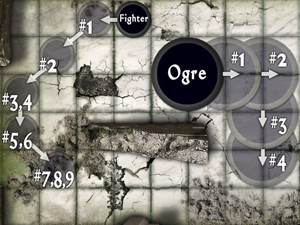
\includegraphics[width=\linewidth]{images/TacticalMovement.jpg}
 The fighter's first move costs him 5 feet (or 1 square). His next costs 5 feet also, but his third (his 2nd diagonal) costs him 10 feet. Next he moves into difficult terrain, also costing him 10 feet. At this point (\#6), the fighter has moved 30 feet---one move action. The last square is a diagonal move in difficult terrain, which costs 15 feet; he must spend his turn's standard action to move this far.\newline
The Large ogre's move costs a total of 20 feet worth of movement (or 4 squares). The ogre cannot cut across the corner to get to that location, and must fully move around it, as indicated.
\end{figure}

\section{Big And Little Creatures In Combat}

\begin{table}[]
\sffamily
\caption{Table: Creature Size and Scale}
\begin{tabular}{lll}
\textbf{Creature Size} & \textbf{Space} & \textbf{Natural Reach*}\\
Fine & 1/2 ft. & 0 \\
 Diminutive & 1 ft. & 0 \\
 Tiny & 2-1/2 ft. & 0 \\
 Small & 5 ft. & 5 ft. \\
 Medium & 5 ft. & 5 ft. \\
 Large (tall) & 10 ft. & 10 ft. \\
 Large (long) & 10 ft. & 5 ft. \\
 Huge (tall) & 15 ft. & 15 ft. \\
 Huge (long) & 15 ft. & 10 ft. \\
 Gargantuan (tall) & 20 ft. & 20 ft. \\
 Gargantuan (long) & 20 ft. & 15 ft. \\
 Colossal (tall) & 30 ft. & 30 ft. \\
 Colossal (long) & 30 ft. & 20 ft.\\
\end{tabular}\\
* These values are typical for creatures of the indicated size. Some exceptions exist.\\
\end{table}
				
Creatures smaller than Small or larger than Medium have special rules relating to position. 
				
\textbf{Tiny, Diminutive, and Fine Creatures}: Very small creatures take up less than 1 square of space. This means that more than one such creature can fit into a single square. A Tiny creature typically occupies a space only 2-1/2 feet across, so four can fit into a single square. 25 Diminutive creatures or 100 Fine creatures can fit into a single square. Creatures that take up less than 1 square of space typically have a natural reach of 0 feet, meaning they can't reach into adjacent squares. They must enter an opponent's square to attack in melee. This provokes an attack of opportunity from the opponent. You can attack into your own square if you need to, so you can attack such creatures normally. Since they have no natural reach, they do not threaten the squares around them. You can move past them without provoking attacks of opportunity. They also can't flank an enemy.
				
\textbf{Large, Huge, Gargantuan, and Colossal Creatures}: Very large creatures take up more than 1 square.
				
Creatures that take up more than 1 square typically have a natural reach of 10 feet or more, meaning that they can reach targets even if they aren't in adjacent squares.
				
Unlike when someone uses a reach weapon, a creature with greater than normal natural reach (more than 5 feet) still threatens squares adjacent to it. A creature with greater than normal natural reach usually gets an attack of opportunity against you if you approach it, because you must enter and move within the range of its reach before you can attack it. This attack of opportunity is not provoked if you take a 5-foot step.
				
Large or larger creatures using reach weapons can strike up to double their natural reach but can't strike at their natural reach or less. 
				
\section{Combat Modifiers}


\begin{table}[]
\sffamily
\caption{Table: Attack Roll Modifiers}
\begin{tabular}{lll}
\textbf{Attacker is...} & \textbf{Melee} & \textbf{Ranged}\\
Dazzled & --1 & --1\\
Entangled & --2 & --2\\
Flanking defender & +2 & —\\
Invisible & +2 & +2\\
On higher ground & +1 & +0\\
Prone & --4 & —\\
Shaken, frightened & --2 & --2\\
Squeezing through a space & --4 & --4\\
\end{tabular}\\
\textsuperscript{1} An entangled character also takes a --4 penalty to Dexterity, which may affect his attack roll.\\
\textsuperscript{2} The defender loses any Dexterity bonus to AC.\\
\textsuperscript{3} Most ranged weapons can't be used while the attacker is prone, but you can use a crossbow or shuriken while prone at no penalty.\\
\end{table}

\begin{table}[]
\sffamily
\caption{Table: Armor Class Modifiers}
\begin{tabular}{lll}
\textbf{Defender is…} & \textbf{Melee} & \textbf{Ranged}\\
Behind cover & +4 & +4\\
Blinded & --2\(^{1}\) & --2\(^{1}\)\\
Concealed or  & See Concealment\\
Cowering & --2\(^{1}\) & --2\(^{1}\)\\
Entangled & +0\(^{2}\) & +0\(^{2}\)\\
Flat-footed & +0\(^{1}\) & +0\(^{1}\)\\
Grappling (but attacker is not) & +0 & +0\\
Helpless & --4\(^{3}\) & +0\(^{3}\)\\
Kneeling or sitting & --2 & +2\\
Pinned & --4\(^{3}\) & +0\(^{3}\)\\
Prone & --4 & +4\\
Squeezing through a space & --4 & --4\\
Stunned & --2\(^{1}\) & --2\(^{1}\)\\
\end{tabular}\\
\textsuperscript{1} The defender loses any Dexterity bonus to AC.\\
\textsuperscript{2} An entangled character takes a --4 penalty to Dexterity.\\
\textsuperscript{3} The defender is denied his Dexterity bonus to his Armor Class.\\
\end{table}


A number of factors and conditions can influence an attack roll. Many of these situations grant a bonus or penalty on attack rolls or to a defender's Armor Class.

\subsection{Cover}

				
To determine whether your target has cover from your ranged attack, choose a corner of your square. If any line from this corner to any corner of the target's square passes through a square or border that blocks line of effect or provides cover, or through a square occupied by a creature, the target has cover (+4 to AC).
				
When making a melee attack against an adjacent target, your target has cover if any line from any corner of your square to the target's square goes through a wall (including a low wall). When making a melee attack against a target that isn't adjacent to you (such as with a reach weapon), use the rules for determining cover from ranged attacks.
				
\textbf{Low Obstacles and Cover}: A low obstacle (such as a wall no higher than half your height) provides cover, but only to creatures within 30 feet (6 squares) of it. The attacker can ignore the cover if he's closer to the obstacle than his target.
				
\textbf{Cover and Attacks of Opportunity}: You can't execute an attack of opportunity against an opponent with cover relative to you.
				
\textbf{Cover and Reflex Saves}: Cover grants you a +2 bonus on Reflex saves against attacks that originate or burst out from a point on the other side of the cover from you. Note that spread effects can extend around corners and thus negate this cover bonus.
				
\textbf{Cover and Stealth Checks}: You can use cover to make a Stealth check. Without cover, you usually need concealment (see below) to make a Stealth check.
				
\textbf{Soft Cover}: Creatures, even your enemies, can provide you with cover against ranged attacks, giving you a +4 bonus to AC. However, such soft cover provides no bonus on Reflex saves, nor does soft cover allow you to make a Stealth check.
				
\textbf{Big Creatures and Cover}: Any creature with a space larger than 5 feet (1 square) determines cover against melee attacks slightly differently than smaller creatures do. Such a creature can choose any square that it occupies to determine if an opponent has cover against its melee attacks. Similarly, when making a melee attack against such a creature, you can pick any of the squares it occupies to determine if it has cover against you.
				
\textbf{Partial Cover}: If a creature has cover, but more than half the creature is visible, its cover bonus is reduced to a +2 to AC and a +1 bonus on Reflex saving throws. This partial cover is subject to the GM's discretion.
				
\textbf{Total Cover}: If you don't have line of effect to your target (that is, you cannot draw any line from your square to your target's square without crossing a solid barrier), he is considered to have total cover from you. You can't make an attack against a target that has total cover.
				
\textbf{Improved Cover}: In some cases, such as attacking a target hiding behind an arrowslit, cover may provide a greater bonus to AC and Reflex saves. In such situations, the normal cover bonuses to AC and Reflex saves can be doubled (to +8 and +4, respectively). A creature with this improved cover effectively gains improved evasion against any attack to which the Reflex save bonus applies. Furthermore, improved cover provides a +10 bonus on Stealth checks.

\begin{figure}
\sffamily
\caption{Cover}
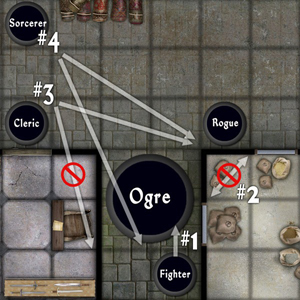
\includegraphics[width=\linewidth]{images/Cover.jpg}
\#1: The fighter is adjacent to the ogre, and nothing blocks him from reaching it. The ogre does not have cover against the fighter.\newline
\#2: The rogue is adjacent to the ogre, but lines from the corners of her square to the corners of the ogre's square cross through a wall. The ogre has melee cover from her, but if it attacks her, the rogue does not have cover from it, as the ogre has reach (so it figures attacks as if attacking with a ranged weapon).\newline
\#3: The cleric attacks at range, and must pick one of the corners of her square to determine cover. Some of these lines pass through a solid surface, meaning that the ogre has cover.\newline
\#4: The sorcerer attacks at range as well, but her lines reveal that she can clearly see more than half of the ogre. This gives the ogre partial cover.
\end{figure}

				
\subsection{Concealment}

				
To determine whether your target has concealment from your ranged attack, choose a corner of your square. If any line from this corner to any corner of the target's square passes through a square or border that provides concealment, the target has concealment.
				
When making a melee attack against an adjacent target, your target has concealment if his space is entirely within an effect that grants concealment. When making a melee attack against a target that isn't adjacent to you, use the rules for determining concealment from ranged attacks.
				
In addition, some magical effects provide concealment against all attacks, regardless of whether any intervening concealment exists.
				
\textbf{Concealment Miss Chance}: Concealment gives the subject of a successful attack a 20\% chance that the attacker missed because of the concealment. Make the attack normally---if the attacker hits, the defender must make a miss chance d\% roll to avoid being struck. Multiple concealment conditions do not stack.
				
\textbf{Concealment and Stealth Checks}: You can use concealment to make a Stealth check. Without concealment, you usually need cover to make a Stealth check.
				
\textbf{Total Concealment}: If you have line of effect to a target but not line of sight, he is considered to have total concealment from you. You can't attack an opponent that has total concealment, though you can attack into a square that you think he occupies. A successful attack into a square occupied by an enemy with total concealment has a 50\% miss chance (instead of the normal 20\% miss chance for an opponent with concealment).
				
You can't execute an attack of opportunity against an opponent with total concealment, even if you know what square or squares the opponent occupies.
				
\textbf{Ignoring Concealment}: Concealment isn't always effective. An area of dim lighting or darkness doesn't provide any concealment against an opponent with darkvision. Characters with low-light vision can see clearly for a greater distance than other characters with the same light source. Although \textit{invisibility} provides total concealment, sighted opponents may still make Perception checks to notice the location of an invisible character. An invisible character gains a +20 bonus on Stealth checks if moving, or a +40 bonus on Stealth checks when not moving (even though opponents can't see you, they might be able to figure out where you are from other visual or auditory clues).
				
\textbf{Varying Degrees of Concealment}: Certain situations may provide more or less than typical concealment, and modify the miss chance accordingly.
				
\subsection{Flanking}

				
When making a melee attack, you get a +2 flanking bonus if your opponent is threatened by another enemy character or creature on its opposite border or opposite corner.
				
When in doubt about whether two characters flank an opponent in the middle, trace an imaginary line between the two attackers' centers. If the line passes through opposite borders of the opponent's space (including corners of those borders), then the opponent is flanked.
				
\textit{Exception}: If a flanker takes up more than 1 square, it gets the flanking bonus if any square it occupies counts for flanking.
				
Only a creature or character that threatens the defender can help an attacker get a flanking bonus.
				
Creatures with a reach of 0 feet can't flank an opponent.

\begin{figure}
\sffamily
\caption{Flanking}
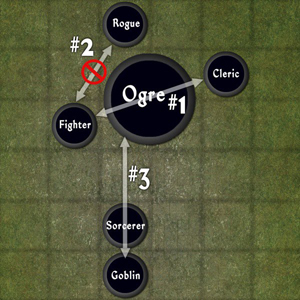
\includegraphics[width=\linewidth]{images/Flanking.jpg}
\#1: The fighter and the cleric are flanking the ogre because they can draw a line to each other that passes through opposite sides of the ogre. Both the fighter and the cleric receive a +2 bonus on attack rolls made against the ogre.\newline
\#2: The rogue is not flanking the ogre because she cannot draw a line to the fighter or the cleric that passes through opposite sides of the ogre. The rogue cannot draw a line to the sorcerer because the sorcerer is not adjacent to the ogre and does not threaten it.\newline
\#3: The goblin and the ogre flank the sorcerer, as they can draw a line between them that passes through opposite sides of the sorcerer's square. If the ogre didn't have reach to the sorcerer, though, he and the goblin would not be flanking her.
\end{figure}

\subsection{Helpless Defenders}

				
A helpless opponent is someone who is bound, sleeping, paralyzed, unconscious, or otherwise at your mercy.
				
\textbf{Regular Attack}: A helpless character takes a --4 penalty to AC against melee attacks. In addition, a helpless character is treated as having a Dexterity of 0, giving him a --5 penalty to AC against both melee and ranged attacks (for a total of --9 against melee and --5 against ranged). A helpless character is also flat-footed.
				
\textbf{Coup de Grace}: As a full-round action, you can use a melee weapon to deliver a coup de grace (pronounced \texttt{{}"{}}coo day grahs\texttt{{}"{}}) to a helpless opponent. You can also use a bow or crossbow, provided you are adjacent to the target. 
				
You automatically hit and score a critical hit. If the defender survives the damage, he must make a Fortitude save (DC 10 + damage dealt) or die. A rogue also gets her extra sneak attack damage against a helpless opponent when delivering a coup de grace.
				
Delivering a coup de grace provokes attacks of opportunity from threatening opponents.
				
You can't deliver a coup de grace against a creature that is immune to critical hits. You can deliver a coup de grace against a creature with total concealment, but doing this requires two consecutive full-round actions (one to \texttt{{}"{}}find\texttt{{}"{}} the creature once you've determined what square it's in, and one to deliver the coup de grace).
				
\section{Special Attacks}

				
This section discusses all of the various standard maneuvers you can perform during combat other than normal attacks, casting spells, or using other class abilities. Some of these special attacks can be made as part of another action (such as an attack) or as an attack of opportunity.
				
\subsection{Aid Another}

				
In melee combat, you can help a friend attack or defend by distracting or interfering with an opponent. If you're in position to make a melee attack on an opponent that is engaging a friend in melee combat, you can attempt to aid your friend as a standard action. You make an attack roll against AC 10. If you succeed, your friend gains either a +2 bonus on his next attack roll against that opponent or a +2 bonus to AC against that opponent's next attack (your choice), as long as that attack comes before the beginning of your next turn. Multiple characters can aid the same friend, and similar bonuses stack.
				
You can also use this standard action to help a friend in other ways, such as when he is affected by a spell, or to assist another character's skill check.
				
\subsection{Charge}

				
Charging is a special full-round action that allows you to move up to twice your speed and attack during the action. Charging, however, carries tight restrictions on how you can move.
				
\textbf{Movement During a Charge}: You must move before your attack, not after. You must move at least 10 feet (2 squares) and may move up to double your speed directly toward the designated opponent. If you move a distance equal to your speed or less, you can also draw a weapon during a charge attack if your base attack bonus is at least +1.
				
You must have a clear path toward the opponent, and nothing can hinder your movement (such as difficult terrain or obstacles). You must move to the closest space from which you can attack the opponent. If this space is occupied or otherwise blocked, you can't charge. If any line from your starting space to the ending space passes through a square that blocks movement, slows movement, or contains a creature (even an ally), you can't charge. Helpless creatures don't stop a charge.
				
If you don't have line of sight to the opponent at the start of your turn, you can't charge that opponent.
				
You can't take a 5-foot step in the same round as a charge.
				
If you are able to take only a standard action on your turn, you can still charge, but you are only allowed to move up to your speed (instead of up to double your speed) and you cannot draw a weapon unless you possess the Quick Draw feat. You can't use this option unless you are restricted to taking only a standard action on your turn.
				
\textbf{Attacking on a Charge}: After moving, you may make a single melee attack. You get a +2 bonus on the attack roll and take a --2 penalty to your AC until the start of your next turn.
				
A charging character gets a +2 bonus on combat maneuver attack rolls made to bull rush an opponent.
				
Even if you have extra attacks, such as from having a high enough base attack bonus or from using multiple weapons, you only get to make one attack during a charge.
				
\textbf{Lances and Charge Attacks}: A lance deals double damage if employed by a mounted character in a charge.
				
\textbf{Weapons Readied against a Charge}: Spears, tridents, and other weapons with the brace feature deal double damage when readied (set) and used against a charging character.
				
\subsection{Combat Maneuvers}

				
During combat, you can attempt to perform a number of maneuvers that can hinder or even cripple your foe, including bull rush, disarm, grapple, overrun, sunder, and trip. Although these maneuvers have vastly different results, they all use a similar mechanic to determine success.
				
\textbf{Combat Maneuver Bonus}: Each character and creature has a Combat Maneuver Bonus (or CMB) that represents its skill at performing combat maneuvers. A creature's CMB is determined using the following formula:
				
{\large \textbf{CMB = Base attack bonus + Strength modifier + special size modifier}}
				
Creatures that are size Tiny or smaller use their Dexterity modifier in place of their Strength modifier to determine their CMB. The special size modifier for a creature's Combat Maneuver Bonus is as follows: Fine --8, Diminutive --4, Tiny --2, Small --1, Medium +0, Large +1, Huge +2, Gargantuan +4, Colossal +8. Some feats and abilities grant a bonus to your CMB when performing specific maneuvers.
				
\textbf{Performing a Combat Maneuver}: When performing a combat maneuver, you must use an action appropriate to the maneuver you are attempting to perform. While many combat maneuvers can be performed as part of an attack action, full-attack action, or attack of opportunity (in place of a melee attack), others require a specific action. Unless otherwise noted, performing a combat maneuver provokes an attack of opportunity from the target of the maneuver. If you are hit by the target, you take the damage normally and apply that amount as a penalty to the attack roll to perform the maneuver. If your target is immobilized, unconscious, or otherwise incapacitated, your maneuver automatically succeeds (treat as if you rolled a natural 20 on the attack roll). If your target is stunned, you receive a +4 bonus on your attack roll to perform a combat maneuver against it. 
				
When you attempt to perform a combat maneuver, make an attack roll and add your CMB in place of your normal attack bonus. Add any bonuses you currently have on attack rolls due to spells, feats, and other effects. These bonuses must be applicable to the weapon or attack used to perform the maneuver. The DC of this maneuver is your target's Combat Maneuver Defense. Combat maneuvers are attack rolls, so you must roll for concealment and take any other penalties that would normally apply to an attack roll.
				
\textbf{Combat Maneuver Defense}: Each character and creature has a Combat Maneuver Defense (or CMD) that represents its ability to resist combat maneuvers. A creature's CMD is determined using the following formula:

{\large \textbf{CMD = 10 + Base attack bonus + Strength modifier + Dexterity modifier + special size modifier}}
				
The special size modifier for a creature's Combat Maneuver Defense is as follows: Fine --8, Diminutive --4, Tiny --2, Small --1, Medium +0, Large +1, Huge +2, Gargantuan +4, Colossal +8. Some feats and abilities grant a bonus to your CMD when resisting specific maneuvers. A creature can also add any circumstance, deflection, dodge, insight, luck, morale, profane, and sacred bonuses to AC to its CMD. Any penalties to a creature's AC also apply to its CMD. A flat-footed creature does not add its Dexterity bonus to its CMD.
				
\textbf{Determine Success}: If your attack roll equals or exceeds the CMD of the target, your maneuver is a success and has the listed effect. Some maneuvers, such as bull rush, have varying levels of success depending on how much your attack roll exceeds the target's CMD. Rolling a natural 20 while attempting a combat maneuver is always a success (except when attempting to escape from bonds), while rolling a natural 1 is always a failure.
				
\subsection{Bull Rush}

				
You can make a bull rush as a standard action or as part of a charge, in place of the melee attack. You can only bull rush an opponent who is no more than one size category larger than you. A bull rush attempts to push an opponent straight back without doing any harm. If you do not have the Improved Bull Rush feat, or a similar ability, initiating a bull rush provokes an attack of opportunity from the target of your maneuver.
				
If your attack is successful, your target is pushed back 5 feet. For every 5 by which your attack exceeds your opponent's CMD you can push the target back an additional 5 feet. You can move with the target if you wish but you must have the available movement to do so. If your attack fails, your movement ends in front of the target.
				
An enemy being moved by a bull rush does not provoke an attack of opportunity because of the movement unless you possess the Greater Bull Rush feat. You cannot bull rush a creature into a square that is occupied by a solid object or obstacle. If there is another creature in the way of your bull rush, you must immediately make a combat maneuver check to bull rush that creature. You take a --4 penalty on this check for each creature being pushed beyond the first. If you are successful, you can continue to push the creatures a distance equal to the lesser result. For example, if a fighter bull rushes a goblin for a total of 15 feet, but there is another goblin 5 feet behind the first, he must make another combat maneuver check against the second goblin after having pushed the first 5 feet. If his check reveals that he can push the second goblin a total of 20 feet, he can continue to push both goblins another 10 feet (since the first goblin will have moved a total of 15 feet).
				
\subsection{Disarm}

				
You can attempt to disarm your opponent in place of a melee attack. If you do not have the Improved Disarm feat, or a similar ability, attempting to disarm a foe provokes an attack of opportunity from the target of your maneuver. Attempting to disarm a foe while unarmed imposes a --4 penalty on the attack.
				
If your attack is successful, your target drops one item it is carrying of your choice (even if the item is wielded with two hands). If your attack exceeds the CMD of the target by 10 or more, the target drops the items it is carrying in both hands (maximum two items if the target has more than two hands). If your attack fails by 10 or more, you drop the weapon that you were using to attempt the disarm. If you successfully disarm your opponent without using a weapon, you may automatically pick up the item dropped.
				
\subsection{Grapple}

				
As a standard action, you can attempt to grapple a foe, hindering his combat options. If you do not have Improved Grapple, grab, or a similar ability, attempting to grapple a foe provokes an attack of opportunity from the target of your maneuver. Humanoid creatures without two free hands attempting to grapple a foe take a --4 penalty on the combat maneuver roll. If successful, both you and the target gain the grappled condition (see the Appendices). If you successfully grapple a creature that is not adjacent to you, move that creature to an adjacent open space (if no space is available, your grapple fails). Although both creatures have the grappled condition, you can, as the creature that initiated the grapple, release the grapple as a free action, removing the condition from both you and the target. If you do not release the grapple, you must continue to make a check each round, as a standard action, to maintain the hold. If your target does not break the grapple, you get a +5 circumstance bonus on grapple checks made against the same target in subsequent rounds. Once you are grappling an opponent, a successful check allows you to continue grappling the foe, and also allows you to perform one of the following actions (as part of the standard action spent to maintain the grapple).
				
\textit{Move}: You can move both yourself and your target up to half your speed. At the end of your movement, you can place your target in any square adjacent to you. If you attempt to place your foe in a hazardous location, such as in a \textit{wall of fire} or over a pit, the target receives a free attempt to break your grapple with a +4 bonus.
				
\textit{Damage}: You can inflict damage to your target equal to your unarmed strike, a natural attack, or an attack made with armor spikes or a light or one-handed weapon. This damage can be either lethal or nonlethal.
				
\textit{Pin}: You can give your opponent the pinned condition (see Conditions). Despite pinning your opponent, you still only have the grappled condition, but you lose your Dexterity bonus to AC.
				
\textit{Tie Up}: If you have your target pinned, otherwise restrained, or unconscious, you can use rope to tie him up. This works like a pin effect, but the DC to escape the bonds is equal to 20 + your Combat Maneuver Bonus (instead of your CMD). The ropes do not need to make a check every round to maintain the pin. If you are grappling the target, you can attempt to tie him up in ropes, but doing so requires a combat maneuver check at a --10 penalty. If the DC to escape from these bindings is higher than 20 + the target's CMB, the target cannot escape from the bonds, even with a natural 20 on the check.
				
\textbf{If You Are Grappled}: If you are grappled, you can attempt to break the grapple as a standard action by making a combat maneuver check (DC equal to your opponent's CMD; this does not provoke an attack of opportunity) or Escape Artist check (with a DC equal to your opponent's CMD). If you succeed, you break the grapple and can act normally. Alternatively, if you succeed, you can become the grappler, grappling the other creature (meaning that the other creature cannot freely release the grapple without making a combat maneuver check, while you can). Instead of attempting to break or reverse the grapple, you can take any action that doesn't require two hands to perform, such as cast a spell or make an attack or full attack with a light or one-handed weapon against any creature within your reach, including the creature that is grappling you. See the grappled condition for additional details. If you are pinned, your actions are very limited. See the pinned condition in Conditions for additional details.
				
\textbf{Multiple Creatures}: Multiple creatures can attempt to grapple one target. The creature that first initiates the grapple is the only one that makes a check, with a +2 bonus for each creature that assists in the grapple (using the Aid Another action). Multiple creatures can also assist another creature in breaking free from a grapple, with each creature that assists (using the Aid Another action) granting a +2 bonus on the grappled creature's combat maneuver check.
				
\subsection{Overrun}

				
As a standard action, taken during your move or as part of a charge, you can attempt to overrun your target, moving through its square. You can only overrun an opponent who is no more than one size category larger than you. If you do not have the Improved Overrun feat, or a similar ability, initiating an overrun provokes an attack of opportunity from the target of your maneuver. If your overrun attempt fails, you stop in the space directly in front of the opponent, or the nearest open space in front of the creature if there are other creatures occupying that space.
				
When you attempt to overrun a target, it can choose to avoid you, allowing you to pass through its square without requiring an attack. If your target does not avoid you, make a combat maneuver check as normal. If your maneuver is successful, you move through the target's space. If your attack exceeds your opponent's CMD by 5 or more, you move through the target's space and the target is knocked prone. If the target has more than two legs, add +2 to the DC of the combat maneuver attack roll for each additional leg it has.
				
\subsection{Sunder}

				
You can attempt to sunder an item held or worn by your opponent as part of an attack action in place of a melee attack. If you do not have the Improved Sunder feat, or a similar ability, attempting to sunder an item provokes an attack of opportunity from the target of your maneuver. 
				
If your attack is successful, you deal damage to the item normally. Damage that exceeds the object's Hardness is subtracted from its hit points. If an object has equal to or less than half its total hit points remaining, it gains the broken condition (see Conditions). If the damage you deal would reduce the object to less than 0 hit points, you can choose to destroy it. If you do not choose to destroy it, the object is left with only 1 hit point and the broken condition.
				
\subsection{Trip}

				
You can attempt to trip your opponent in place of a melee attack. You can only trip an opponent who is no more than one size category larger than you. If you do not have the Improved Trip feat, or a similar ability, initiating a trip provokes an attack of opportunity from the target of your maneuver.
				
If your attack exceeds the target's CMD, the target is knocked prone. If your attack fails by 10 or more, you are knocked prone instead. If the target has more than two legs, add +2 to the DC of the combat maneuver attack roll for each additional leg it has. Some creatures---such as oozes, creatures without legs, and flying creatures---cannot be tripped.
				
\subsection{Feint}

				
Feinting is a standard action. To feint, make a Bluff skill check. The DC of this check is equal to 10 + your opponent's base attack bonus + your opponent's Wisdom modifier. If your opponent is trained in Sense Motive, the DC is instead equal to 10 + your opponent's Sense Motive bonus, if higher. If successful, the next melee attack you make against the target does not allow him to use his Dexterity bonus to AC (if any). This attack must be made on or before your next turn.
				
When feinting against a nonhumanoid you take a --4 penalty. Against a creature of animal Intelligence (1 or 2), you take a --8 penalty. Against a creature lacking an Intelligence score, it's impossible. Feinting in combat does not provoke attacks of opportunity.
				
\textbf{Feinting as a Move Action}: With the Improved Feint feat, you can attempt a feint as a move action.
				
\subsection{Mounted Combat}

				
These rules cover being mounted on a horse in combat but can also be applied to more unusual steeds, such as a griffon or dragon.
				
\textbf{Mounts in Combat}: Horses, ponies, and riding dogs can serve readily as combat steeds. Mounts that do not possess combat training (see the Handle Animal skill) are frightened by combat. If you don't dismount, you must make a DC 20 Ride check each round as a move action to control such a mount. If you succeed, you can perform a standard action after the move action. If you fail, the move action becomes a full-round action, and you can't do anything else until your next turn.
				
Your mount acts on your initiative count as you direct it. You move at its speed, but the mount uses its action to move.
				
A horse (not a pony) is a Large creature and thus takes up a space 10 feet (2 squares) across. For simplicity, assume that you share your mount's space during combat.
				
\textbf{Combat while Mounted}: With a DC 5 Ride check, you can guide your mount with your knees so as to use both hands to attack or defend yourself. This is a free action.
				
When you attack a creature smaller than your mount that is on foot, you get the +1 bonus on melee attacks for being on higher ground. If your mount moves more than 5 feet, you can only make a single melee attack. Essentially, you have to wait until the mount gets to your enemy before attacking, so you can't make a full attack. Even at your mount's full speed, you don't take any penalty on melee attacks while mounted.
				
If your mount charges, you also take the AC penalty associated with a charge. If you make an attack at the end of the charge, you receive the bonus gained from the charge. When charging on horseback, you deal double damage with a lance (see Charge).
				
You can use ranged weapons while your mount is taking a double move, but at a --4 penalty on the attack roll. You can use ranged weapons while your mount is running (quadruple speed) at a --8 penalty. In either case, you make the attack roll when your mount has completed half its movement. You can make a full attack with a ranged weapon while your mount is moving. Likewise, you can take move actions normally.
				
\textbf{Casting Spells While Mounted}: You can cast a spell normally if your mount moves up to a normal move (its speed) either before or after you cast. If you have your mount move both before and after you cast a spell, then you're casting the spell while the mount is moving, and you have to make a concentration check due to the vigorous motion (DC 10 + spell level) or lose the spell. If the mount is running (quadruple speed), you can cast a spell when your mount has moved up to twice its speed, but your concentration check is more difficult due to the violent motion (DC 15 + spell level).
				
\textbf{If Your Mount Falls in Battle}: If your mount falls, you have to succeed on a DC 15 Ride check to make a soft fall and take no damage. If the check fails, you take 1d6 points of damage.
				
\textbf{If You Are Dropped}: If you are knocked unconscious, you have a 50\% chance to stay in the saddle (75\% if you're in a military saddle). Otherwise you fall and take 1d6 points of damage. Without you to guide it, your mount avoids combat.
				
\subsection{Throw Splash Weapon}

				
A splash weapon is a ranged weapon that breaks on impact, splashing or scattering its contents over its target and nearby creatures or objects. To attack with a splash weapon, make a ranged touch attack against the target. Thrown splash weapons require no weapon proficiency, so you don't take the --4 nonproficiency penalty. A hit deals direct hit damage to the target, and splash damage to all creatures within 5 feet of the target. If the target is Large or larger, you choose one of its squares and the splash damage affects creatures within 5 feet of that square. Splash weapons cannot deal precision-based damage (such as sneak attack). 
				
You can instead target a specific grid intersection. Treat this as a ranged attack against AC 5. However, if you target a grid intersection, creatures in all adjacent squares are dealt the splash damage, and the direct hit damage is not dealt to any creature. You can't target a grid intersection occupied by a creature, such as a Large or larger creature; in this case, you're aiming at the creature.
				
If you miss the target (whether aiming at a creature or a grid intersection), roll 1d8. This determines the misdirection of the throw, with 1 falling short (off-target in a straight line toward the thrower), and 2 through 8 rotating around the target creature or grid intersection in a clockwise direction. Then, count a number of squares in the indicated direction equal to the range increment of the throw. After you determine where the weapon landed, it deals splash damage to all creatures in that square and in all adjacent squares.
				
\subsection{Two-Weapon Fighting}

				
If you wield a second weapon in your off hand, you can get one extra attack per round with that weapon. You suffer a --6 penalty with your regular attack or attacks with your primary hand and a --10 penalty to the attack with your off hand when you fight this way. You can reduce these penalties in two ways. First, if your off-hand weapon is light, the penalties are reduced by 2 each. An unarmed strike is always considered light. Second, the Two-Weapon Fighting feat lessens the primary hand penalty by 2, and the off-hand penalty by 6.
				
Table: Two-weapon Fighting Penalties summarizes the interaction of all these factors.
				
\textbf{Double Weapons}: You can use a double weapon to make an extra attack with the off-hand end of the weapon as if you were fighting with two weapons. The penalties apply as if the off-hand end of the weapon was a light weapon.
				
\textbf{Thrown Weapons}: The same rules apply when you throw a weapon from each hand. Treat a dart or shuriken as a light weapon when used in this manner, and treat a bolas, javelin, net, or sling as a one-handed weapon.

\begin{table}[]
\sffamily
\caption{Table: Two-Weapon Fighting Penalties}
\begin{tabular}{lll}
\textbf{Circumstances} & \textbf{Primary Hand} & \textbf{Off Hand}\\
Normal penalties & --6 & --10\\
Off-hand weapon is light & --4 & --8\\
Two-Weapon Fighting feat & --4 & --4\\
Off-hand weapon is light and  & --2 & --2\\
Two-Weapon Fighting feat & \\
\end{tabular}
\end{table}

\section{Special Initiative Actions}

				
Here are ways to change when you act during combat by altering your place in the initiative order.
				
\subsection{Delay}

				
By choosing to delay, you take no action and then act normally on whatever initiative count you decide to act. When you delay, you voluntarily reduce your own initiative result for the rest of the combat. When your new, lower initiative count comes up later in the same round, you can act normally. You can specify this new initiative result or just wait until some time later in the round and act then, thus fixing your new initiative count at that point.
				
You never get back the time you spend waiting to see what's going to happen. You also can't interrupt anyone else's action (as you can with a readied action).
				
\textbf{Initiative Consequences of Delaying}: Your initiative result becomes the count on which you took the delayed action. If you come to your next action and have not yet performed an action, you don't get to take a delayed action (though you can delay again).
				
If you take a delayed action in the next round, before your regular turn comes up, your initiative count rises to that new point in the order of battle, and you do not get your regular action that round.
				
\subsection{Ready}

				
The ready action lets you prepare to take an action later, after your turn is over but before your next one has begun. Readying is a standard action. It does not provoke an attack of opportunity (though the action that you ready might do so).
				
\textbf{Readying an Action}: You can ready a standard action, a move action, a swift action, or a free action. To do so, specify the action you will take and the conditions under which you will take it. Then, anytime before your next action, you may take the readied action in response to that condition. The action occurs just before the action that triggers it. If the triggered action is part of another character's activities, you interrupt the other character. Assuming he is still capable of doing so, he continues his actions once you complete your readied action. Your initiative result changes. For the rest of the encounter, your initiative result is the count on which you took the readied action, and you act immediately ahead of the character whose action triggered your readied action.
				
You can take a 5-foot step as part of your readied action, but only if you don't otherwise move any distance during the round. 
				
\textbf{Initiative Consequences of Readying}: Your initiative result becomes the count on which you took the readied action. If you come to your next action and have not yet performed your readied action, you don't get to take the readied action (though you can ready the same action again). If you take your readied action in the next round, before your regular turn comes up, your initiative count rises to that new point in the order of battle, and you do not get your regular action that round.
				
\textbf{Distracting Spellcasters}: You can ready an attack against a spellcaster with the trigger \texttt{{}"{}}if she starts casting a spell.\texttt{{}"{}} If you damage the spellcaster, she may lose the spell she was trying to cast (as determined by her concentration check result).
				
\textbf{Readying to Counterspell}: You may ready a counterspell against a spellcaster (often with the trigger \texttt{{}"{}}if she starts casting a spell\texttt{{}"{}}). In this case, when the spellcaster starts a spell, you get a chance to identify it with a Spellcraft check (DC 15 + spell level). If you do, and if you can cast that same spell (and are able to cast it and have it prepared, if you prepare spells), you can cast the spell as a counterspell and automatically ruin the other spellcaster's spell. Counterspelling works even if one spell is divine and the other arcane.
				
A spellcaster can use \textit{dispel magic }to counterspell another spellcaster, but it doesn't always work.
				
\textbf{Readying a Weapon against a Charge}: You can ready weapons with the brace feature, setting them to receive charges. A readied weapon of this type deals double damage if you score a hit with it against a charging character.
			
% </div id="ready">
        	
